%% BioMed_Central_Tex_Template_v1.06
%%                                      %
%  bmc_article.tex            ver: 1.06 %
%                                       %

%%IMPORTANT: do not delete the first line of this template
%%It must be present to enable the BMC Submission system to
%%recognise this template!!

%%%%%%%%%%%%%%%%%%%%%%%%%%%%%%%%%%%%%%%%%
%%                                     %%
%%  LaTeX template for BioMed Central  %%
%%     journal article submissions     %%
%%                                     %%
%%          <8 June 2012>              %%
%%                                     %%
%%                                     %%
%%%%%%%%%%%%%%%%%%%%%%%%%%%%%%%%%%%%%%%%%


%%%%%%%%%%%%%%%%%%%%%%%%%%%%%%%%%%%%%%%%%%%%%%%%%%%%%%%%%%%%%%%%%%%%%
%%                                                                 %%
%% For instructions on how to fill out this Tex template           %%
%% document please refer to Readme.html and the instructions for   %%
%% authors page on the biomed central website                      %%
%% http://www.biomedcentral.com/info/authors/                      %%
%%                                                                 %%
%% Please do not use \input{...} to include other tex files.       %%
%% Submit your LaTeX manuscript as one .tex document.              %%
%%                                                                 %%
%% All additional figures and files should be attached             %%
%% separately and not embedded in the \TeX\ document itself.       %%
%%                                                                 %%
%% BioMed Central currently use the MikTex distribution of         %%
%% TeX for Windows) of TeX and LaTeX.  This is available from      %%
%% http://www.miktex.org                                           %%
%%                                                                 %%
%%%%%%%%%%%%%%%%%%%%%%%%%%%%%%%%%%%%%%%%%%%%%%%%%%%%%%%%%%%%%%%%%%%%%

%%% additional documentclass options:
%  [doublespacing]
%  [linenumbers]   - put the line numbers on margins

%%% loading packages, author definitions

%\documentclass[twocolumn]{bmcart}% uncomment this for twocolumn layout and comment line below
\documentclass{bmcart}

%%% Load packages
%\usepackage{amsthm,amsmath}
%\RequirePackage{natbib}
%\RequirePackage[authoryear]{natbib}% uncomment this for author-year bibliography
%\RequirePackage{hyperref}
\usepackage[utf8]{inputenc} %unicode support
%\usepackage[applemac]{inputenc} %applemac support if unicode package fails
%\usepackage[latin1]{inputenc} %UNIX support if unicode package fails

\usepackage{graphicx}

%%%%%%%%%%%%%%%%%%%%%%%%%%%%%%%%%%%%%%%%%%%%%%%%%
%%                                             %%
%%  If you wish to display your graphics for   %%
%%  your own use using includegraphic or       %%
%%  includegraphics, then comment out the      %%
%%  following two lines of code.               %%
%%  NB: These line *must* be included when     %%
%%  submitting to BMC.                         %%
%%  All figure files must be submitted as      %%
%%  separate graphics through the BMC          %%
%%  submission process, not included in the    %%
%%  submitted article.                         %%
%%                                             %%
%%%%%%%%%%%%%%%%%%%%%%%%%%%%%%%%%%%%%%%%%%%%%%%%%




%%% Put your definitions there:
\startlocaldefs
\endlocaldefs


%%% Begin ...
\begin{document}

%%% Start of article front matter
\begin{frontmatter}

\begin{fmbox}
\dochead{Research}

%%%%%%%%%%%%%%%%%%%%%%%%%%%%%%%%%%%%%%%%%%%%%%
%%                                          %%
%% Enter the title of your article here     %%
%%                                          %%
%%%%%%%%%%%%%%%%%%%%%%%%%%%%%%%%%%%%%%%%%%%%%%

\title{Consistent Multiple Nonnegative Matrix Factorization with Hierarchical Information for Gene Functional Modules Mining}

%%%%%%%%%%%%%%%%%%%%%%%%%%%%%%%%%%%%%%%%%%%%%%
%%                                          %%
%% Enter the authors here                   %%
%%                                          %%
%% Specify information, if available,       %%
%% in the form:                             %%
%%   <key>={<id1>,<id2>}                    %%
%%   <key>=                                 %%
%% Comment or delete the keys which are     %%
%% not used. Repeat \author command as much %%
%% as required.                             %%
%%                                          %%
%%%%%%%%%%%%%%%%%%%%%%%%%%%%%%%%%%%%%%%%%%%%%%

\author[
   addressref={aff1},                   % id's of addresses, e.g. {aff1,aff2}
   corref={aff1},                       % id of corresponding address, if any
   noteref={n1},                        % id's of article notes, if any
   email={jane.e.doe@cambridge.co.uk}   % email address
]{\inits{JE}\fnm{Jane E} \snm{Doe}}
\author[
   addressref={aff1,aff2},
   email={john.RS.Smith@cambridge.co.uk}
]{\inits{JRS}\fnm{John RS} \snm{Smith}}

%%%%%%%%%%%%%%%%%%%%%%%%%%%%%%%%%%%%%%%%%%%%%%
%%                                          %%
%% Enter the authors' addresses here        %%
%%                                          %%
%% Repeat \address commands as much as      %%
%% required.                                %%
%%                                          %%
%%%%%%%%%%%%%%%%%%%%%%%%%%%%%%%%%%%%%%%%%%%%%%

\address[id=aff1]{%                           % unique id
  \orgname{Department of Zoology, Cambridge}, % university, etc
  \street{Waterloo Road},                     %
  %\postcode{}                                % post or zip code
  \city{London},                              % city
  \cny{UK}                                    % country
}
\address[id=aff2]{%
  \orgname{Marine Ecology Department, Institute of Marine Sciences Kiel},
  \street{D\"{u}sternbrooker Weg 20},
  \postcode{24105}
  \city{Kiel},
  \cny{Germany}
}

%%%%%%%%%%%%%%%%%%%%%%%%%%%%%%%%%%%%%%%%%%%%%%
%%                                          %%
%% Enter short notes here                   %%
%%                                          %%
%% Short notes will be after addresses      %%
%% on first page.                           %%
%%                                          %%
%%%%%%%%%%%%%%%%%%%%%%%%%%%%%%%%%%%%%%%%%%%%%%

\begin{artnotes}
%\note{Sample of title note}     % note to the article
\note[id=n1]{Equal contributor} % note, connected to author
\end{artnotes}

\end{fmbox}% comment this for two column layout

%%%%%%%%%%%%%%%%%%%%%%%%%%%%%%%%%%%%%%%%%%%%%%
%%                                          %%
%% The Abstract begins here                 %%
%%                                          %%
%% Please refer to the Instructions for     %%
%% authors on http://www.biomedcentral.com  %%
%% and include the section headings         %%
%% accordingly for your article type.       %%
%%                                          %%
%%%%%%%%%%%%%%%%%%%%%%%%%%%%%%%%%%%%%%%%%%%%%%

\begin{abstractbox}

\begin{abstract} % abstract
\parttitle{First part title} %if any
Mining gene functional modules in the whole genome has great significance which may provide clues about the main biological processes and mechanism of genetic diseases. Nonnegative matrix factorization (NMF) has been successfully used for clustering genes for its good performance and interpretability. However, in some applications, there exists a defined hierarchical architecture behind the data (e.g. phenotype ontology) which is ignored by previous studies. In this paper, we propose a consistent multiple nonnegative matrix factorization (CMNMF) method to address this issue. The CMNMF method constraints the gene clusters to consistence while communicating with phenotypes from different levels of ontology hierarchy and restricts the clusters of phenotypes to fit the hierarchical structure of phenotype ontology. Experiments show the ability of the proposed method to identify gene functional modules with biological significance over the baseline methods.

\parttitle{Second part title} %if any
Text for this section.
\end{abstract}

%%%%%%%%%%%%%%%%%%%%%%%%%%%%%%%%%%%%%%%%%%%%%%
%%                                          %%
%% The keywords begin here                  %%
%%                                          %%
%% Put each keyword in separate \kwd{}.     %%
%%                                          %%
%%%%%%%%%%%%%%%%%%%%%%%%%%%%%%%%%%%%%%%%%%%%%%

\begin{keyword}
\kwd{sample}
\kwd{article}
\kwd{author}
\end{keyword}

% MSC classifications codes, if any
%\begin{keyword}[class=AMS]
%\kwd[Primary ]{}
%\kwd{}
%\kwd[; secondary ]{}
%\end{keyword}

\end{abstractbox}
%
%\end{fmbox}% uncomment this for twcolumn layout

\end{frontmatter}

%%%%%%%%%%%%%%%%%%%%%%%%%%%%%%%%%%%%%%%%%%%%%%
%%                                          %%
%% The Main Body begins here                %%
%%                                          %%
%% Please refer to the instructions for     %%
%% authors on:                              %%
%% http://www.biomedcentral.com/info/authors%%
%% and include the section headings         %%
%% accordingly for your article type.       %%
%%                                          %%
%% See the Results and Discussion section   %%
%% for details on how to create sub-sections%%
%%                                          %%
%% use \cite{...} to cite references        %%
%%  \cite{koon} and                         %%
%%  \cite{oreg,khar,zvai,xjon,schn,pond}    %%
%%  \nocite{smith,marg,hunn,advi,koha,mouse}%%
%%                                          %%
%%%%%%%%%%%%%%%%%%%%%%%%%%%%%%%%%%%%%%%%%%%%%%

%%%%%%%%%%%%%%%%%%%%%%%%% start of article main body
% <put your article body there>

%%%%%%%%%%%%%%%%
%% Background %%
%%
\section*{Introduction}
It is significant to discover gene functional modules in the whole genome, which may help to select related genes in the main biological processes associated to different physiological states and identify candidate genes of genetic diseases. In recent decade, NMF and series of varieties have been successfully adopted for clustering on gene-phenotype association data because of its good interpretability and stable performance \cite{document_cluster_NMF,cluster_bwk}, in which relations between phenotype are not considered. However, the hierarchical structure of phenotype ontology is ignored, although it has been the main representation of phenotypes.

To make full use of the structure information behind the data, some structure based methods are proposed and all achieve good results. SNMNMF tried to integrate multiple type genomic data to identify microRNA-gene regulatory modules \cite{SMNMF}. In collaborative recommendation task, some grouping strategies by the defined hierarchy are proposed \cite{SoRec,HMF,HGMF}. HPMF focusd on predicting missing traits for plants which incorporates hierarchical phylogenetic information into matrix factorization \cite{HPMF}. The results of these methods demonstrate that incorporating stucture information can bring a better performance.

In this work, we assume that genes can be annotated with phenotype ontologies from different levels (or granularity) of hierarchy, but the clustering of these genes with different representation should be consistent. Motivated by it, we propose a NMF-based method called CMNMF (consistent multiple non-negative matrix factorization) for gene functional modules mining, in which the hierarchical structure of phenotype is used as prior knowledge. In detail, a consistent constraint on gene clusters and a hierarchical mapping constraint on phenotype ontologies are adopted in the loss function. In addition, a sparse constraint on gene-phenotype associations is added in the regularized version. Experiment on simulated data illustrates how our CMNMF uses hierarchical structure and experiments on biological data show the ability of CMNMF to mining gene functional modules with biological significance.


\section*{Method}
Given a binary matrix $A_{(m \times n)}$ denotes gene-phenotype associations by $m$ genes and $n$ phenotypes, where $A_{ij}$ is set to 1 for a known association and 0 otherwise. The goal of factorizing matrix $A$ is to derive gene functional clusters based on gene-phenotype associations. The loss of it can be defined as $min _{P,G} ||A-GP||^{2}_{F}$, where G and P denotes gene clusters and phenotype clusters, respectively.

However, the NMF in this form cannot make full use of the hierarchical mapping information of phenotype ontology. To address this problem, we design a loss function with two components for formulating the loss with hierarchical information of phenotype ontologies. The first component is a consistent constraint on gene clusters, we restrict the gene clustering results on parent and child phenotype ontology levels should be consistent(See Fig.\ref{fig:cmnmf}(a)). The second component is a hierarchical mapping constraint with phenotype ontologies from parent level and child level, as shown in Fig.\ref{fig:cmnmf}(b). With it, the clusters of phenotype ontologies from different levels should fit the hierarchical architecture. By optimizing these two components, a CMNMF (Consistent Multiple Non-negative Matrix Factorization) algorithm is proposed to obtain consistent gene clusters.
\begin{figure}
\centering
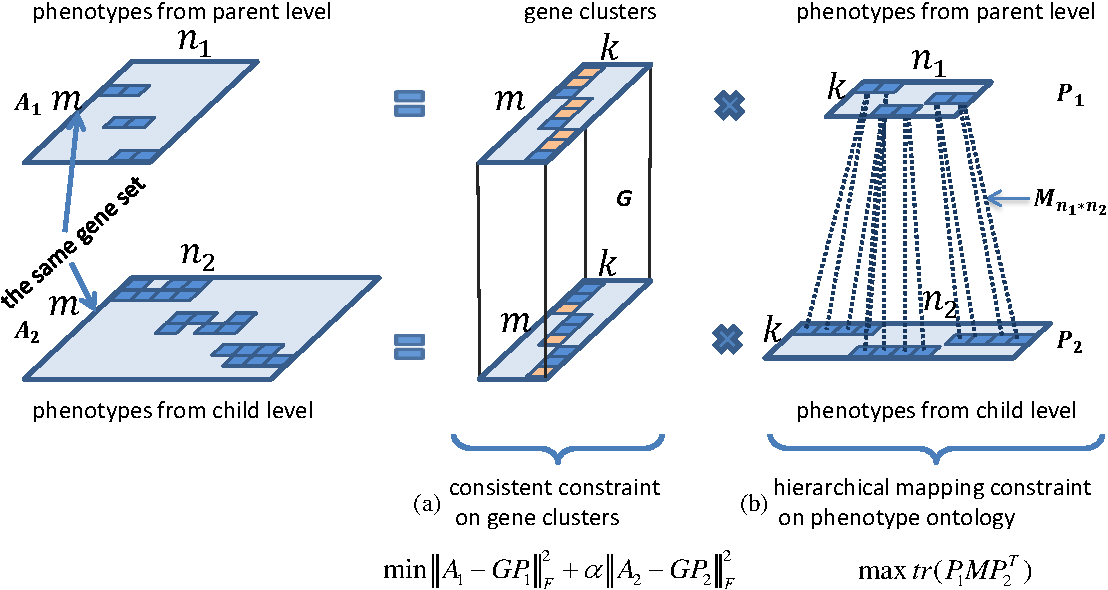
\includegraphics[width=4in]{fig/model.pdf}
\caption{Overview of the proposed CMNMF model}
\label{fig:cmnmf}
\end{figure}

\subsection*{Loss Functions for Penalizing Inconsistence}

Motivated by the consistent assumption, we extract phenotype ontologies from two adjacent levels, and  denote them as parent level and child level. Correspondingly, two gene-phenotype association matrices $A_{1}$ and $A_{2}$ are extracted according to two extracted sets of phenotype ontologies and all genes. We assume that the factorizations on $A_{1}$ and $A_{2}$ for the same gene set should be consistent, although the gene are annotated by phenotype ontologies from parent levels and child levels, respectively. In our work, factorized $G_{1}$ and $G_{2}$ should be same. Hence, we use the same $G$ in two terms of matrix factorization. The following quadratic function can be used to model the first loss:
\begin{equation}
\label{eqn:LC}
{L_C} = \mathop {\min }\limits_{G,{P_1},{P_2}} \left\| {{A_1} - G{P_1}} \right\|_F^2 + \alpha \left\| {{A_2} - G{P_2}} \right\|_F^2,
\end{equation}
where $\alpha$ is a parameter to balance the factorization error from different levels, $G$ is gene clusters and $P_1$ and $P_2$ are the clusters of phenotypes from different levels.

For the hierarchical mapping constraint on phenotype ontologies from parent level and child level, loss function in Eq.(\ref{eqn:LH}) is used to encourage the consistence between phenotype clustering in parent level and child level.
\begin{equation}
\label{eqn:LH}
{L_H} = \sum\limits_{ij} {{M_{ij}}} {(p_1^{(i)})^T}p_2^{(j)} = tr({P_1}MP_2^T),\
\end{equation}
where matrix $M$ denotes the hierarchical mapping relations between phenotype ontologies from different levels.  The $M_{ij}=1$, if phenotype $i$ and phenotype $j$ have a parent-child relationship, otherwise 0. We enforce hierarchical mapping constraints by maximizing the mapping between the phenotype ontologies in gene-phenotype network $A_{1}$ and $A_{2}$.


\subsection*{Regularization by Sparse Constraint}
Since the known gene-phenotype associations are sparse and only cover a part of genes and phenotypes, the regularization with $L_2-norm$ is proposed to control the sparseness of $G$, $P_1$ and $P_2$. The term ${\lambda _1}\|G\|_F^2$ limits the sharing of genes in different gene functional modules. The term ${\lambda _2}(\| {{P_1}}\|_F^2+\|P_2\|_F^2)$ also encourages the sparsity of phenotype clusters. Finally, the loss function of CMNMF with sparse constraint and non-negative constraint is listed as follows:
\begin{equation}
\label{eqn:cmnmf}
\begin{array}{l}
\mathop {\min }\limits_{G,{P_1},{P_2}} \left\| {{A_1} - G{P_1}} \right\|_F^2 + \alpha \left\| {{A_2} - G{P_2}} \right\|_F^2 - \gamma tr({P_1}MP_2^T)\\
\quad\quad\quad{\rm{ + }}{\lambda _1}\left\| G \right\|_F^2{\rm{ + }}{\lambda _2}(\left\| {{P_1}} \right\|_F^2{\rm{ + }}\left\| {{P_2}} \right\|_F^2)\\

s.t.,{\rm{  G}} \ge {\rm{0, }}{{\rm{P}}_1}{\rm{ }} {{\rm{P}}_2} \ge 0
\end{array}\;
\end{equation}
where $\alpha ,\gamma ,{\lambda _1},{\lambda _2}$ are parameters to balance the trade of each component.

\subsection*{The CMNMF Algorithm}
To minimize the loss function in Eq.(\ref{eqn:cmnmf}), we have developed an algorithm CMNMF that can optimize the objective function iteratively by fixing one variable alternatively. As in the original NMF model, the cost function (\ref{eqn:cmnmf}) is not convex in $G$ and $P$ jointly, but it is convex in $G$ for fixed $P_1$ and $P_2$, vice versa, the Lagrange multiplier method can be applicable here to give an iterative algorithm to guarantee the algorithm to converge to a local minima \cite{document_cluster_NMF}.

To solve the equation Eq.(\ref{eqn:cmnmf}), let $\Phi ,\Psi ,\Omega $ be the Lagrange multipliers for nonnegative constraint for $G$, $P_1$ and $P_2$, then the augmented Lagrangian can be written as formula \ref{eqn:lagrange_multiplier}:
\begin{equation}
    \label{eqn:lagrange_multiplier}
    {L(G,{P_1},{P_2})}= J + tr({\Phi}{G^T}) + tr({\Psi}P_1^T) + tr({\Omega}P_2^T)
\end{equation}
When fixing $P_1$ and $P_2$, the partial derivative of L with respect to $G$ is:
\begin{equation}
\label{eqn:derivation}
\frac{{\partial L}}{{\partial G}} =  - 2({A_1}P_1^T - G{P_1}P_1^T) - 2\alpha ({A_2}P_2^T - G{P_2}P_2^T) + 2{\lambda _1}G + \Phi \\\\
\end{equation}
Using the Karush-Kuhn-Tucker (KKT) conditions, $\Phi_{ij}{G_{ij}} = 0$, we can get the following updating rule for G:
\begin{equation}
\label{eqn:update_G}
{G_{ij}} \leftarrow {G_{ij}}\frac{{{{({A_1}P_1^T + \alpha {A_2}P_2^T)}_{ij}}}}{{{{(G{P_1}P_1^T + \alpha G{P_2}P_2^T + {\lambda _1}G)}_{ij}}}}\\\\
\end{equation}

As the same with updating $G$, fixing $G$, the partial derivative of L with respect to $P_1$ and $P_2$ are:
\begin{equation}
\begin{array}{l}
\frac{{\partial L}}{{\partial {P_1}}} =  - 2({G^T}{A_1} - {G^T}G{P_1}) - \gamma {P_2}{M^T} + 2{\lambda _2}{P_1} + \Psi \\\\
\frac{{\partial L}}{{\partial {P_2}}} =  - 2\alpha ({G^T}{A_2} - {G^T}G{P_2}) - \gamma {P_1}M + 2{\lambda _2}{P_2} + \Omega
\end{array}
\end{equation}
then, we get the updating rule for $P_1$ and $P_2$:
\begin{equation}
\begin{array}{l}
(P_1)_{ij} \leftarrow (P_1)_{ij}\frac{{{{({G^T}{A_1} + \frac{1}{2}\gamma {P_2}{M^T})}_{ij}}}}{{({G^T}G{P_1} + {\lambda _2}{P_1}){}_{ij}}}\\\\
(P_2)_{ij} \leftarrow (P_2)_{ij}\frac{{{{(\alpha {G^T}{A_2} + \frac{1}{2}\gamma {P_1}M)}_{ij}}}}{{(\alpha {G^T}G{P_2} + {\lambda _2}{P_2}){}_{ij}}}
\end{array}
\end{equation}

Algorithm 1 describes the iterative algorithm for the CMNMF method.

\makebox{
  \begin{minipage}{0.7\textwidth}
    \textrm{Algorithm CMNMF} \\
    \textrm{Input:} $A_1$,$A_2$,$M$ \\
        parameters: $\alpha, \gamma, \lambda_1, \lambda_2$, MaxIter; \\
    \textrm{Output:} $G$, $P_1$,$P_2$


    \begin{enumerate}
    %    \vspace{-10pt}
        \item[1] {\textrm{\bf{while}} ($t < MaxIter$)\{}
        \item[2] {Update $G$:}
        \item[3] {~~~~ ${G_{ij}} \leftarrow {G_{ij}}\frac{{{{({A_1}P_1^T + \alpha {A_2}P_2^T)}_{ij}}}}{{{{(G{P_1}P_1^T + \alpha G{P_2}P_2^T + {\lambda _1}G)}_{ij}}}}$}
        \item[4] {Update P1 P2 simultaneously:}
        \item[5] {~~~~ $(P_1){_{ij}} \leftarrow (P_1)_{ij}\frac{{{{({G^T}{A_1} + \frac{1}{2}\gamma {P_2}{M^T})}_{ij}}}}{{({G^T}G{P_1} + {\lambda _2}{P_1}){}_{ij}}}$;}
        \item[6] {~~~~ $(P_2)_{ij} \leftarrow (P_2)_{ij}\frac{{{{(\alpha {G^T}{A_2} + \frac{1}{2}\gamma {P_1}M)}_{ij}}}}{{(\alpha {G^T}G{P_2} + {\lambda _2}{P_2}){}_{ij}}}$;}
        \item[7] {\textbf{end while}}

    \end{enumerate}

  \end{minipage}
}


\section*{Experiments and Analysis}
Our method is demonstrated on simulated gene-phenotype association matrixes at first by comparing the difference of conventional NMF and proposed CMNMF. We then execute CMNMF and four baseline methods on MGI mouse gene-phenotype ontology associations for mining mouse gene functional modules. Moreover, the evaluation of clustering results and parameter tuning are performed. Finally, gene ontology enrichment analysis by DAVID is adopted to evaluate the biological significance of mined gene modules.

\subsection*{CMNMF on Simulated Data}
We generated gene-phenotype association matrixes $A_1$, $A_2$ and hierarchical mapping relations $M$ to illustrate the usage of the hierarchical information. Fig.\ref{fig:simulate_data}(a) describes the structure of the simulated data in which genes are assigned into three groups. For each group, there are two genes associating with phenotypes in the child level and another gene associating with the parent phenotypes. The task is to cluster the three genes into a same group. Due to the third gene doesn't have any associated phenotypes in the same level with that another two genes associate with, neither on $A_1$ nor on $A_2$ can NMF group the third gene into a same cluster with another two as shown in Fig.(\ref{fig:simulate_data})(b-1) and Fig.(\ref{fig:simulate_data})(b-2).
\begin{figure}
  \centering
  \begin{minipage}{.4\linewidth}
  \centering
    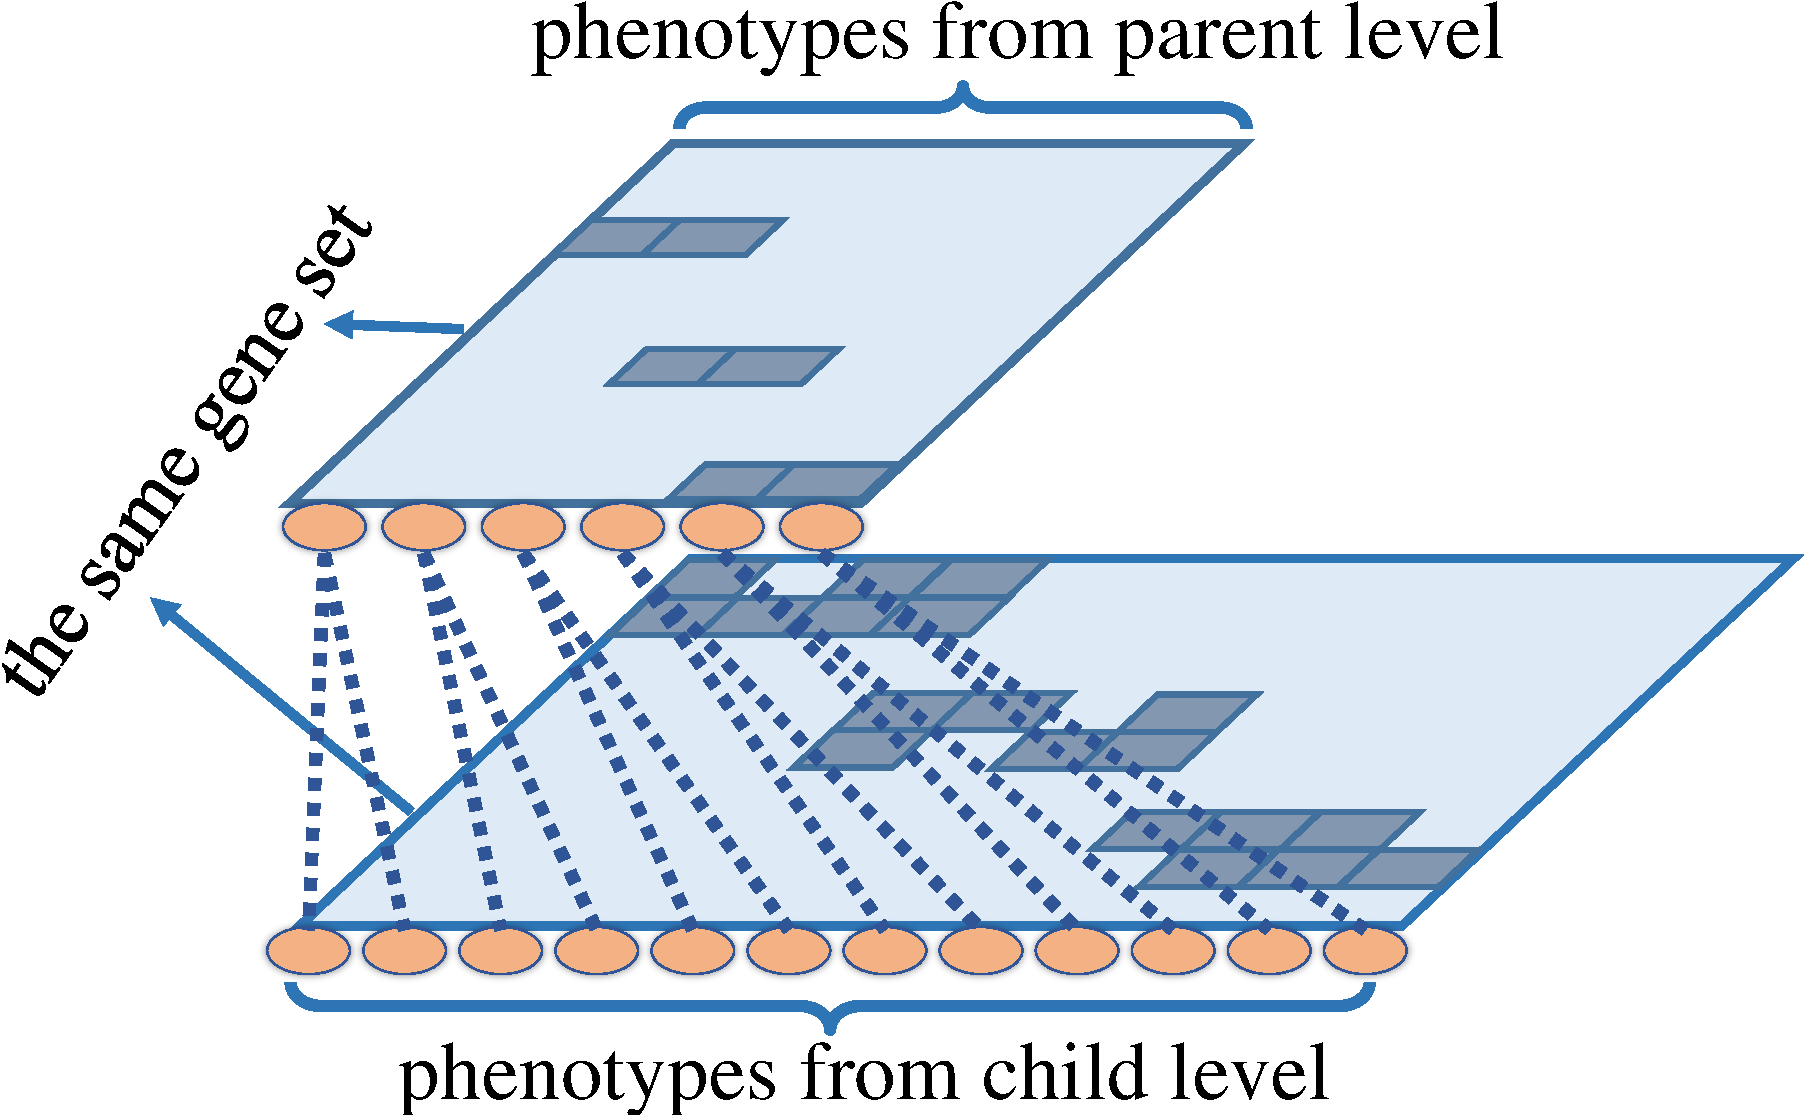
\includegraphics[width=\linewidth]{fig/simulate_data.pdf}
    \centerline{(a)}
  \end{minipage}
  \begin{minipage}{.4\linewidth}
   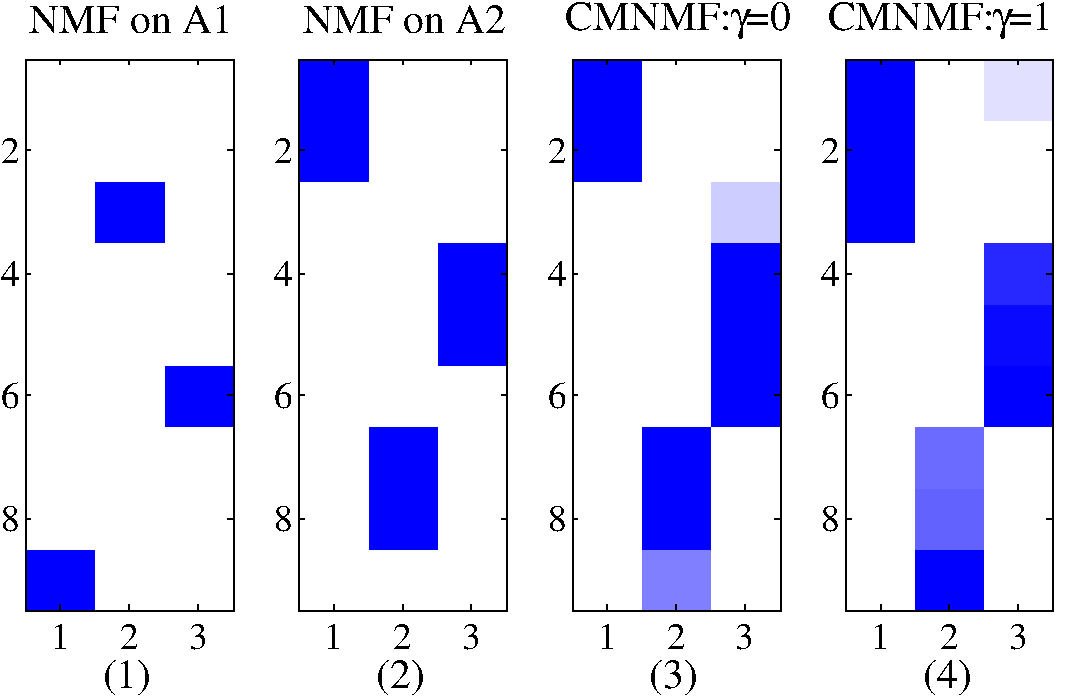
\includegraphics[width=\linewidth]{fig/simulate_result.pdf}
    \centerline{(b)}
  \end{minipage}
  \caption{(a)Hierarchical structure of simulated data, (b) Performance of CMNMF and NMF under different conditions: (b-1) Cluster result of NMF on parent level, (b-2) Cluster result of NMF on child level, (b-3) Cluster result of CMNMF($\gamma$=0), (b-4) Cluster result of CMNMF($\gamma$=1)}
  \label{fig:simulate_data}
\end{figure}

To analyze how the two proposed constraints work, CMNMF is applied to the simulated data to cluster the genes. We first set the parameter $\gamma$ which controls the effect of hierarchical constraint on CMNMF to zero. As shown in Fig.\ref{fig:simulate_data}(b-3), combing information from two levels and restricting the cluster results of genes to remain consistent indeed help improve the performance. But there still exists little misclassification (the third gene in the first group is wrongly assigned to the second group). When introducing the hierarchical constraint ($\gamma$=1) to the model, the CMNMF method groups all the genes into the correct clusters (See Fig.\ref{fig:simulate_data}(b-4)), which demonstrates that the two constraints working together can get the best performance. The reasons for the performance improvement are that with the consistent constraint, CMNMF can incorporate information from two levels and take advantage of the complement characteristic of information from different levels to overcome the shortcoming of lacking enough information from only one level and the hierarchy constraint can help restrict cluster results according with the structure of data which narrows the range of solution space so that we can get a better solution.


\section*{Mining Mouse Gene Functional Modules}
\subsection*{Data Preparation}
In this study, we evaluate the proposed CMNMF and baseline methods on MGI mouse gene-phenotype ontology association data. The mouse gene-phenotype ontology associations are extracted from file ``MGI\_Geno\_Disease.rpt'' (March-2015) downloaded from MGI \footnote[1]{ftp://ftp.informatics.jax.org/pub/reports/MGI\_Geno\_Disease.rpt}, in which 5894 phenotype-gene associations at level 4 and 6817 associations at level 5 are kept. 2144 ontology terms at level 4 (parent level) and 2719 ontology terms at level 5 (child level)  are selected from the 10748 MP terms in the OBO file. 2866 hierarchial mapping relations between phenotypes in level 4 and level 5 are kept as $M$.

To evaluate the performance, we collected 288 pathways from KEGG as the ``ground truth''. Genes in a signal pathway can be considered as a gene functional module (or a gene cluster).

\subsection*{Comparison with Baseline Methods by Mining Gene Modules}
CMNMF is executed to mine gene functional modules and it is compared with the following clustering methods, K-Means, HAC (Hierarchical Agglomerative Clustering) \cite{HAC}, NMF and HMF(Hierarchical Matrix Factorization) \cite{HMF}. To be fair, all matrix factorization-based methods are implemented with sparse and non-negative constraints. We measured the performance by the Jaccard coefficient \cite{cluster_survey}. Higher coefficient indicates better clustering result.

Parameters are tuned by cross-validation for all the competitive methods respectively. For all matrix factorization methods, the balancing parameter of sparse constraints on gene clusters $\lambda_1$ and phenotype clusters $\lambda_2$ are set by the grid \{0.001,0.01,0.1,1,10,20\}. For CMNMF, the weight of factorization on child level $\alpha$ is set from 0.1 to 0.9 with an interval of 0.2 and 1 to 9 with an interval of 2, $\gamma$ is set by the range \{0.0001,0.001,0.01,0.1,1\}. The number of modules k is picked to be 300 for all methods, approximating to the number of KEGG mouse pathways. Initial values of $G$ and $P$ (or $P_1$ and $P_2$) are randomized with value between 0 to 1.

The clustering results are column-normalized by using z-score, and the $G_{ij}$ will be set as 0 if it is less than $3\sigma$. All the methods are repeated ten times with different initial values and average Jaccard coefficients are reported in Fig.\ref{fig:jaccard}. Note that the proposed method performs better than other methods except HAC as shown in Fig.\ref{fig:jaccard}(a). But the range of gene clusters size of HAC is much larger than other methods as shown in Fig.\ref{fig:jaccard}(b). In fact, HAC puts 76.5\% of genes into one cluster and the other clusters share the left genes which brings it a better Jaccard coefficient, but it cannot help to identify significant gene functional modules. Additionally, the standard deviations of all the methods are small, which demonstrates that these methods including our CMNMF are insensitive to the initial values (Fig.\ref{fig:jaccard}(a)).
\begin{figure}
  \centering
  \begin{minipage}{.45\linewidth}
    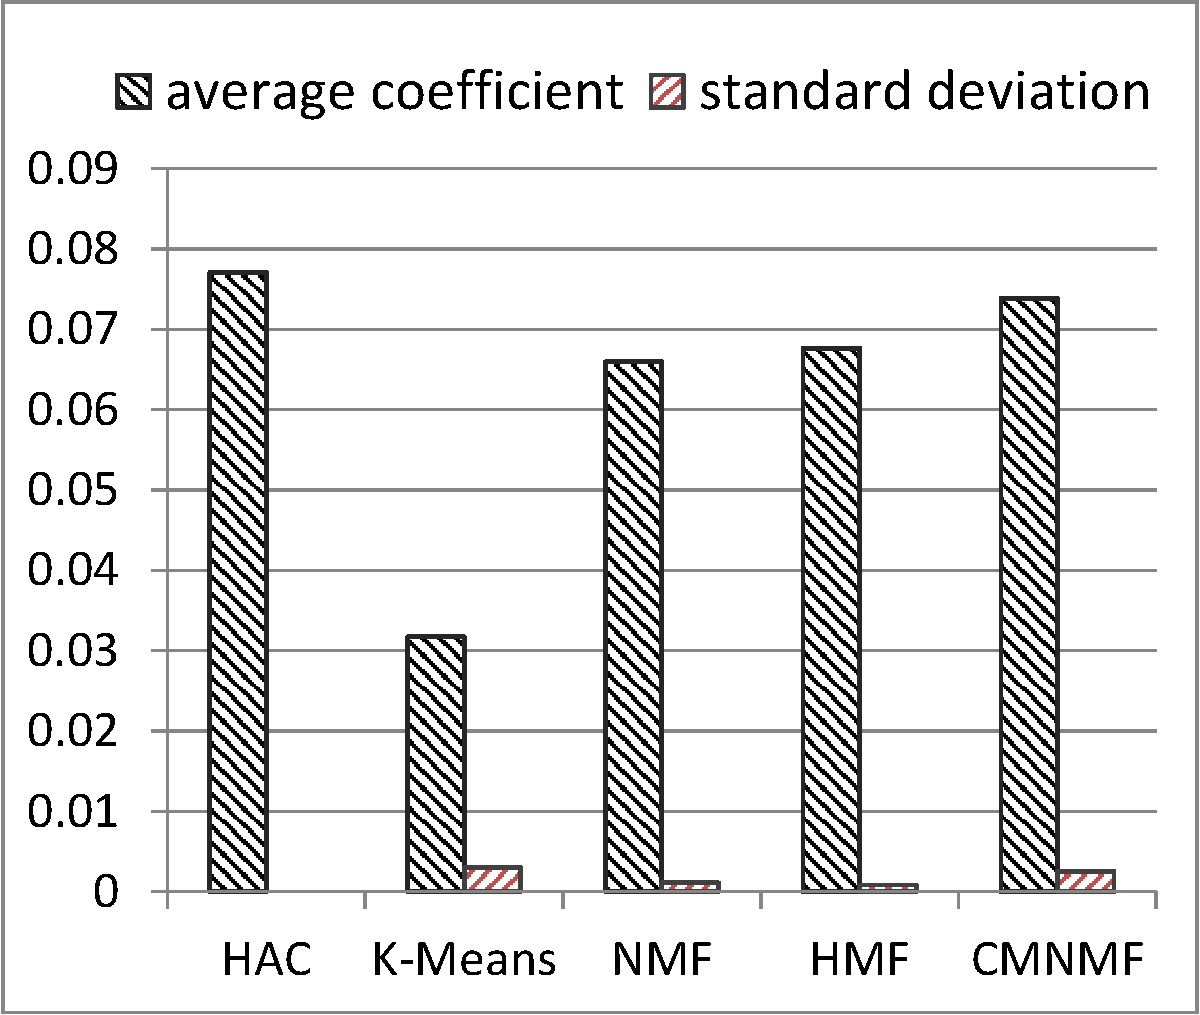
\includegraphics[width=\linewidth]{fig/jaccard.pdf}
    \centerline{(a)}
  \end{minipage}
  \begin{minipage}{.45\linewidth}
   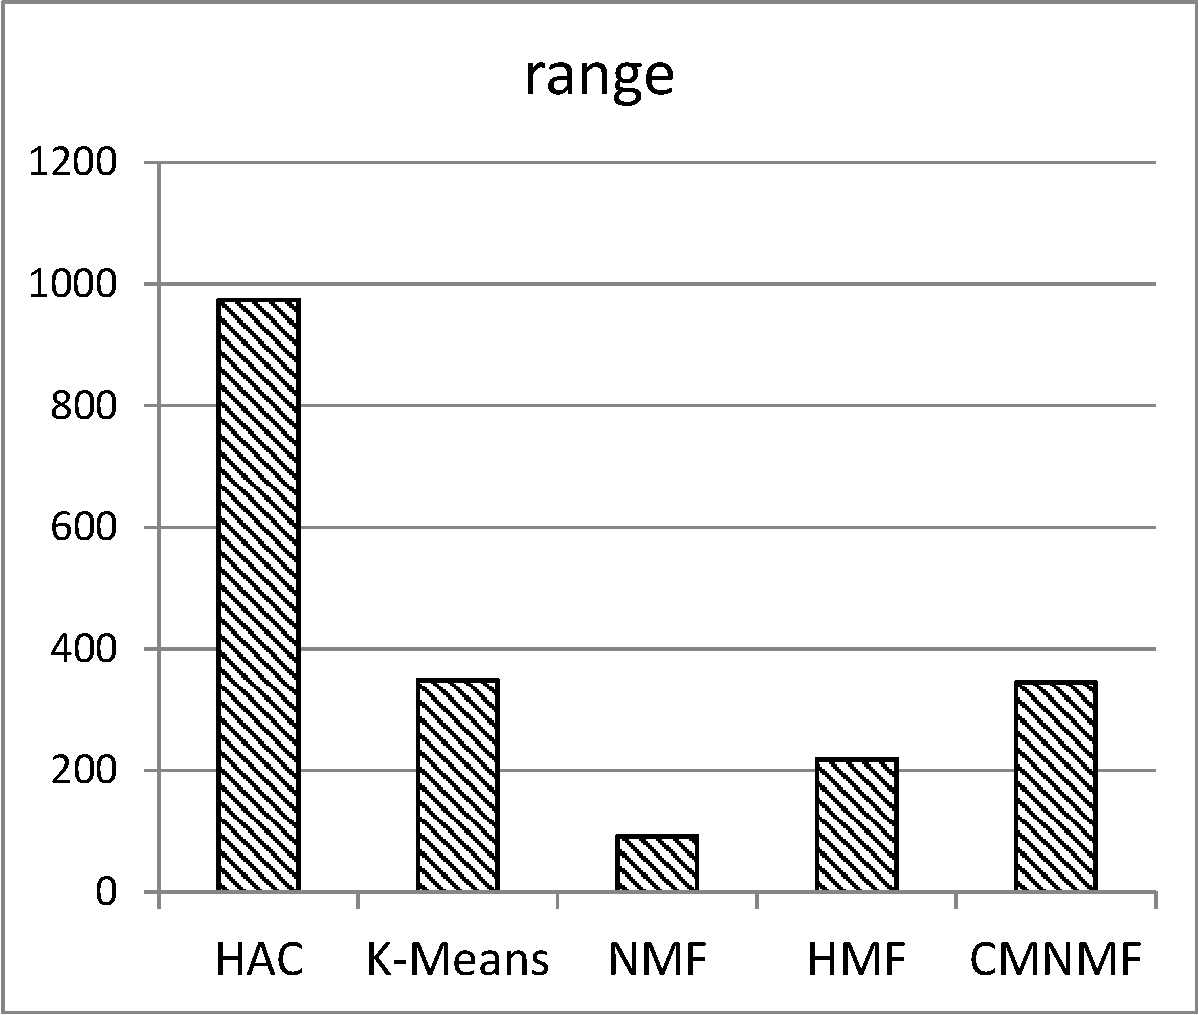
\includegraphics[width=\linewidth]{fig/range.pdf}
    \centerline{(b)}
  \end{minipage}
  \caption{(a) Comparative performance of the proposed method with various methods. (b) Range of gene clusters size of different methods.}
  \label{fig:jaccard}
\end{figure}

The $\alpha$ in our CMNMF model which balances the contributions from different levels is an important parameter. When $\alpha$ is close to 0, the model degenerates into NMF on level 4 and when $\alpha$ is big enough information from level 5 leads the model. The performance of CMNMF with different $\alpha$ is shown in Table \ref{tab:alpha_tune}. We can find that neither $\alpha$ is close to 0 nor big enough the CMNMF model performs best. When $\alpha$ is near 1, our method obtains a best performance which indicates that associations from different levels are mutual complementation with each other and our CMNMF model successfully captures this characteristic.
\begin{table}
\centering
\caption{Performance of CMNMF with different $\alpha$}
\label{tab:alpha_tune}
\begin{tabular}{|c||c|c|c|c|c|c|c|c|c|c|}
\hline
 $\alpha$ &0.1& 0.3&0.5&0.7&0.9&1&3&5&7&9\\
\hline
Jaccard coefficient& 0.056 & 0.059 & 0.066 & 0.063 & \textbf{0.071}& \textbf{0.074} & 0.062 & 0.053 & 0.050 & 0.049\\
\hline
\end{tabular}
\end{table}

\subsection*{GO Enrichment Analysis on Gene Clusters}
We evaluate the biological significance of the identified gene clusters with GO (Gene Ontology) enrichment analysis by DAVID\cite{David}, an online functional annotation tool. It is adopted to analyze a set of genes with annotated gene ontologies in ``biological process''(BP) branch. In general, a large number of annotations means high-quality modules.

In our work, clusters with more than 300 genes and fewer than 5 genes are dropped as suggested in \cite{SMNMF}. Table \ref{tab:go} shows that modules identified by CMNMF have the most GO(BP) terms annotations under different p-value cutoff which demonstrates that our method can mine gene functional modules with more biological significance.

\begin{table}
\centering
\caption{Numbers of GO terms(BP) annotations in the modules under different p-value cutoff to consider a Go term(BP) enriched.}
\label{tab:go}
\begin{tabular}{|c||c|c|c|c|c|}
\hline
 &0.05 & 0.01& 0.001&0.0001&0.00001\\
\hline
\hline
K-Means&46  & 43& 39&38&32\\
\hline
NMF&2399 & 1996&1410&1016&769\\
\hline
HMF&1759& 1479&1030&729&520\\
\hline
CMNMF&\textbf{5586}& \textbf{4691}& \textbf{3594}&\textbf{2706}&\textbf{2090}\\
\hline
\end{tabular}
\end{table}

\section*{Conclusions}
In this paper, we introduce a consistent multiple nonnegative matrix factorization for data with hierarchical information. We first analyze the mechanism of our method on a simulated data, then compare the performance of CMNMF with other methods on mining gene modules. We conclude that the CMNMF method is an effective algorithm which can fully utilize the hierarchical structure information behind the data. Experiments on mining gene functional modules show the ability of CMNMF to identify modules with biological significance. In future, we will try to analyze the expansibility of CMNMF on more than just two levels and try to solve other tasks where data has a hierarchical structure.


%%%%%%%%%%%%%%%%%%%%%%%%%%%%%%%%%%%%%%%%%%%%%%
%%                                          %%
%% Backmatter begins here                   %%
%%                                          %%
%%%%%%%%%%%%%%%%%%%%%%%%%%%%%%%%%%%%%%%%%%%%%%

\begin{backmatter}

\section*{Competing interests}
  The authors declare that they have no competing interests.

\section*{Author's contributions}
    Text for this section \ldots

\section*{Acknowledgements}
This work is supported by the National Natural Science Foundation of China (No. 61300166 and No. 61105049), the Open Project Foundation of Information Technology Research Base of Civil Aviation Administration of China (CAAC-ITRB-201303 and CAAC-ITRB-201408), the Natural Science Foundation of Tianjin (No. 14JCQNJC00600), and the Science and Technology Planning Project of Tianjin (No. 13ZCZDGX01098).

%%%%%%%%%%%%%%%%%%%%%%%%%%%%%%%%%%%%%%%%%%%%%%%%%%%%%%%%%%%%%
%%                  The Bibliography                       %%
%%                                                         %%
%%  Bmc_mathpys.bst  will be used to                       %%
%%  create a .BBL file for submission.                     %%
%%  After submission of the .TEX file,                     %%
%%  you will be prompted to submit your .BBL file.         %%
%%                                                         %%
%%                                                         %%
%%  Note that the displayed Bibliography will not          %%
%%  necessarily be rendered by Latex exactly as specified  %%
%%  in the online Instructions for Authors.                %%
%%                                                         %%
%%%%%%%%%%%%%%%%%%%%%%%%%%%%%%%%%%%%%%%%%%%%%%%%%%%%%%%%%%%%%

% if your bibliography is in bibtex format, use those commands:
\bibliographystyle{bmc-mathphys} % Style BST file (bmc-mathphys, vancouver, spbasic).
\bibliography{bmc_article}      % Bibliography file (usually '*.bib' )
% for author-year bibliography (bmc-mathphys or spbasic)
% a) write to bib file (bmc-mathphys only)
% @settings{label, options="nameyear"}
% b) uncomment next line
%\nocite{label}

% or include bibliography directly:
% \begin{thebibliography}
% \bibitem{b1}
% \end{thebibliography}

%%%%%%%%%%%%%%%%%%%%%%%%%%%%%%%%%%%
%%                               %%
%% Figures                       %%
%%                               %%
%% NB: this is for captions and  %%
%% Titles. All graphics must be  %%
%% submitted separately and NOT  %%
%% included in the Tex document  %%
%%                               %%
%%%%%%%%%%%%%%%%%%%%%%%%%%%%%%%%%%%

%%
%% Do not use \listoffigures as most will included as separate files

\section*{Figures}
  \begin{figure}[h!]
  \caption{\csentence{Sample figure title.}
      A short description of the figure content
      should go here.}
      \end{figure}

\begin{figure}[h!]
  \caption{\csentence{Sample figure title.}
      Figure legend text.}
      \end{figure}

%%%%%%%%%%%%%%%%%%%%%%%%%%%%%%%%%%%
%%                               %%
%% Tables                        %%
%%                               %%
%%%%%%%%%%%%%%%%%%%%%%%%%%%%%%%%%%%

%% Use of \listoftables is discouraged.
%%
\section*{Tables}
\begin{table}[h!]
\caption{Sample table title. This is where the description of the table should go.}
      \begin{tabular}{cccc}
        \hline
           & B1  &B2   & B3\\ \hline
        A1 & 0.1 & 0.2 & 0.3\\
        A2 & ... & ..  & .\\
        A3 & ..  & .   & .\\ \hline
      \end{tabular}
\end{table}

%%%%%%%%%%%%%%%%%%%%%%%%%%%%%%%%%%%
%%                               %%
%% Additional Files              %%
%%                               %%
%%%%%%%%%%%%%%%%%%%%%%%%%%%%%%%%%%%

\section*{Additional Files}
  \subsection*{Additional file 1 --- Sample additional file title}
    Additional file descriptions text (including details of how to
    view the file, if it is in a non-standard format or the file extension).  This might
    refer to a multi-page table or a figure.

  \subsection*{Additional file 2 --- Sample additional file title}
    Additional file descriptions text.


\end{backmatter}
\end{document}
